%
% This is the LaTeX template file for lecture notes for EE 382C/EE 361C.
%
% To familiarize yourself with this template, the body contains
% some examples of its use.  Look them over.  Then you can
% run LaTeX on this file.  After you have LaTeXed this file then
% you can look over the result either by printing it out with
% dvips or using xdvi.
%
% This template is based on the template for Prof. Sinclair's CS 270.

\documentclass[twoside]{article}
\usepackage{graphicx}
\usepackage{wrapfig}
\usepackage{amsmath}
\usepackage{amssymb}
\usepackage{listings}
\setlength{\oddsidemargin}{0.25 in}
\setlength{\evensidemargin}{-0.25 in}
\setlength{\topmargin}{-0.6 in}
\setlength{\textwidth}{6.5 in}
\setlength{\textheight}{8.5 in}
\setlength{\headsep}{0.75 in}
\setlength{\parindent}{0 in}
\setlength{\parskip}{0.1 in}

%
% The following commands set up the lecnum (lecture number)
% counter and make various numbering schemes work relative
% to the lecture number.
%
\newcounter{lecnum}
\renewcommand{\thepage}{\thelecnum-\arabic{page}}
\renewcommand{\thesection}{\thelecnum.\arabic{section}}
\renewcommand{\theequation}{\thelecnum.\arabic{equation}}
\renewcommand{\thefigure}{\thelecnum.\arabic{figure}}
\renewcommand{\thetable}{\thelecnum.\arabic{table}}

%
% The following macro is used to generate the header.
%
\lstset{language=Python, numbers=left, tabsize=2, xleftmargin=5.0ex}

\newcommand{\lecture}[4]{
   \pagestyle{myheadings}
   \thispagestyle{plain}
   \newpage
   \setcounter{lecnum}{#1}
   \setcounter{page}{1}
   \noindent
   \begin{center}
   \framebox{
      \vbox{\vspace{2mm}
    \hbox to 6.28in { {\bf EE 382V: Parallel Algorithms
                        \hfill Summer 2017} }
       \vspace{4mm}
       \hbox to 6.28in { {\Large \hfill Lecture #1: #2  \hfill} }
       \vspace{2mm}
       \hbox to 6.28in { {\it Lecturer: #3 \hfill Scribe: #4} }
      \vspace{2mm}}
   }
   \end{center}
   \markboth{Lecture #1: #2}{Lecture #1: #2}
   %{\bf Disclaimer}: {\it These notes have not been subjected to the
   %usual scrutiny reserved for formal publications.  They may be distributed
   %outside this class only with the permission of the Instructor.}
   \vspace*{4mm}
}

%
% Convention for citations is authors' initials followed by the year.
% For example, to cite a paper by Leighton and Maggs you would type
% \cite{LM89}, and to cite a paper by Strassen you would type \cite{S69}.
% (To avoid bibliography problems, for now we redefine the \cite command.)
% Also commands that create a suitable format for the reference list.
\renewcommand{\cite}[1]{[#1]}
\def\beginrefs{\begin{list}%
        {[\arabic{equation}]}{\usecounter{equation}
         \setlength{\leftmargin}{2.0truecm}\setlength{\labelsep}{0.4truecm}%
         \setlength{\labelwidth}{1.6truecm}}}
\def\endrefs{\end{list}}
\def\bibentry#1{\item[\hbox{[#1]}]}

%Use this command for a figure; it puts a figure in wherever you want it.
%usage: \fig{NUMBER}{SPACE-IN-INCHES}{CAPTION}
\newcommand{\fig}[3]{
			\vspace{#2}
			\begin{center}
			Figure \thelecnum.#1:~#3
			\end{center}
	}
% Use these for theorems, lemmas, proofs, etc.
\newtheorem{theorem}{Theorem}[lecnum]
\newtheorem{lemma}[theorem]{Lemma}
\newtheorem{proposition}[theorem]{Proposition}
\newtheorem{claim}[theorem]{Claim}
\newtheorem{corollary}[theorem]{Corollary}
\newtheorem{definition}[theorem]{Definition}
\newenvironment{proof}{{\bf Proof:}}{\hfill\rule{2mm}{2mm}}

% **** IF YOU WANT TO DEFINE ADDITIONAL MACROS FOR YOURSELF, PUT THEM HERE:

\begin{document}
%FILL IN THE RIGHT INFO.
%\lecture{**LECTURE-NUMBER**}{**DATE**}{**LECTURER**}{**SCRIBE**}
\lecture{21}{July 21}{Vijay Garg}{Abed Haque}
%\footnotetext{These notes are partially based on those of Nigel Mansell.}

% **** YOUR NOTES GO HERE:

% Some general latex examples and examples making use of the
% macros follow.  
%**** IN GENERAL, BE BRIEF. LONG SCRIBE NOTES, NO MATTER HOW WELL WRITTEN,
%**** ARE NEVER READ BY ANYBODY.
\section{Introduction}
During this lecture we covered the following topics:

\begin{itemize}
	\item The Euler Tour Technique
\end{itemize}

This set of lecture notes will briefly re-examine the topics covered in this lecture, in the order in which they appeared during class. 

\section{Euler Tour Technique}
Given some tree, let's say that we want to find the height of the tree.  If it was a balanced tree, this would be easy to do.  But what if the tree was skewed?  The height may not be $log(n)$ in this case.  The Euler Tour Technique is a way to find the height of a tree in $log(n)$ time independent of the height.

Let's think of a linked list as a lopsided tree.  With pointer jumping, we were able to find the length of the linked list in $log(n)$ time.  We can use a similar technique for a tree if we represent it as a linked list.

Given a directed graph, a Euler Tour is a walk along the edges of the graph, starting from any node $v$, in which every edge is traversed exactly once and ends at the vertex $v$.  A graph has an Euler Circuit if and only if every node has an even degree (an even number of edges).

We can view a tree as a linked list of edges.  Let's construct a directed graph from a tree and then define a Euler Tour for the graph.  It is sufficient to specify  the next edge (successor) for every edge $e$ in the directed graph.  Let $v_0 , v_{m-1}$ be the neighbors of $u$.  Then $succ(v_i, u)$ is given by $(u, v_{(i+1\enspace mod\enspace m)})$.  (This is depth first search).

\subsection{Implementation of Euler Tour on a Graph from a Tree} 

Given the tree T shown in Figure \ref{fig:euler1} below, we will construct a Euler Tour.  Figure \ref{fig:euler2} shows the adjacency list representation of the T.  Now let's make two modifications to Figure \ref{fig:euler2}.  First, lets make the lists circular instead of null terminating.  Second, lets put a bidirectional pointer between edges that represents the same undirected edge, represented by a blue dotted line.  This results in the circular adjacency list in Figure \ref{fig:euler3}. 

In this example $succ(1,4) = (4,2)$.  In Figure \ref{fig:euler3}, $succ$ is the element that is shown by the blue dotted edges followed by black edges.  So we can can construct the following Euler Tour directly from Figure \ref{fig:euler3}:

$(1, 4) \rightarrow (4, 2) \rightarrow (2, 4) \rightarrow (4, 3) \rightarrow (3, 4) \rightarrow (4, 1) \rightarrow (1, 5) \rightarrow (5, 1) \rightarrow (1, 4)$

\begin{figure}[!ht]
\centering
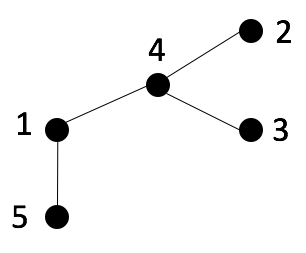
\includegraphics[scale=0.6]{img/EulerCkt1.png}
\caption{A tree T} \label{fig:euler1} 
\end{figure}

\begin{figure}[!ht]
\centering
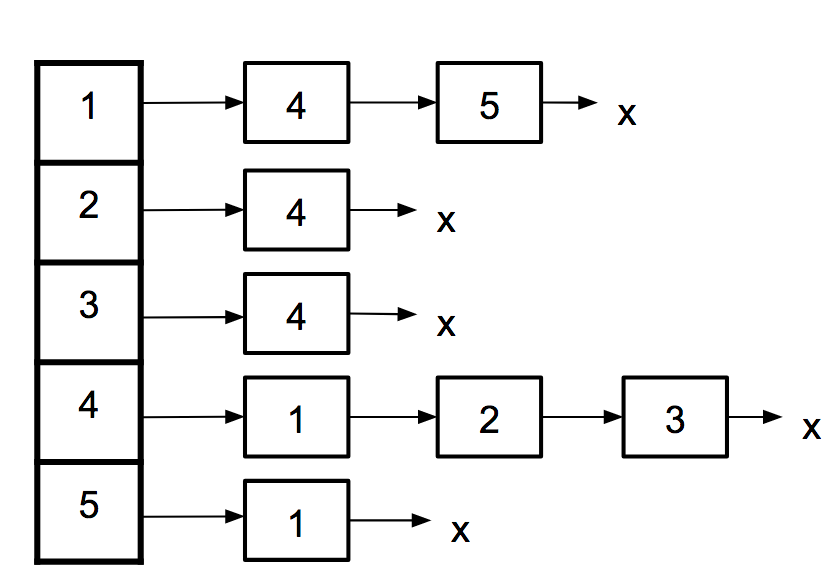
\includegraphics[scale=0.4]{img/EulerCkt2.png}
\caption{The adjacency lists of the tree T} \label{fig:euler2} 
\end{figure}

\begin{figure}[!ht]
\centering
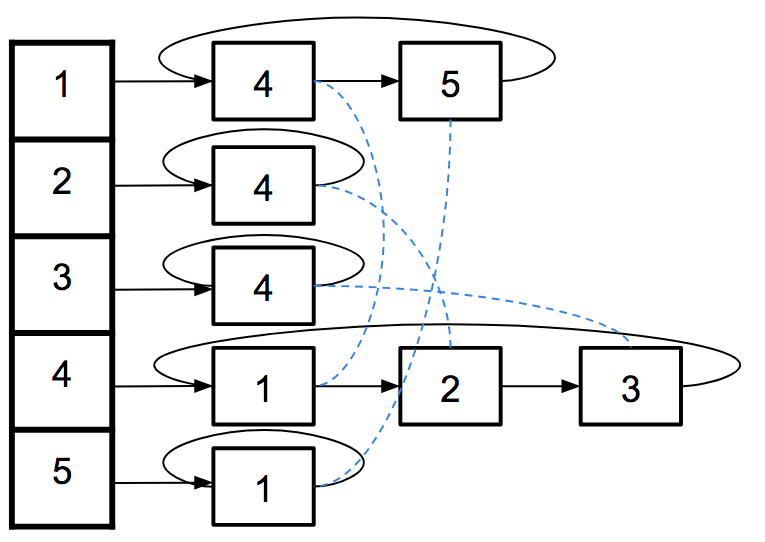
\includegraphics[scale=0.4]{img/Euler3.png}
\caption{The circular adjacency lists of tree T with additional pointers} \label{fig:euler3} 
\end{figure}

\end{document}



Contact GitHub API Training Shop Blog About
� 2017 GitHub, Inc. Terms Privacy Security Status Help